\section{Results}
\label{sec-results}

In this section, we present the results obtained from carrying out our
methodology, and discuss some of the implications of our results. Most of our
results investigate the effect of an independent variable (time-of-day and
developer experience/frequency classifications) on the likelihood of a commit to
be a bug-introducing commit, or \emph{bugginess}. We also describe our findings
with respect to the day of the week, which allows us to compare our results to
those in~\cite{sliwerski-msr-2005}. We also discuss our finding that some
bug-fixing commits only changed comments. Finally, we explain the precision and
recall of our methodology and how we computed these figures.

\subsection{Project Characteristics}
\label{sec-proj-char}

We chose two large open-source software repositories for our investigations:
Linus Torvalds's mainline Linux kernel %, from \url{git.kernel.org} 
and PostgreSQL. %, from the project's repository at \url{git.postgresql.org}.
%
Table~\ref{tab:characteristics} summarizes the characteristics of our
repositories. The row ``lines of code'' refers to the current size of
the code in the repository. The row ``\# bug-introducing'' shows that
23.7--25.5\% of the commits are buggy, which is slightly lower than the
previously reported figure of nearly 40\% for a commercial switching
system~\cite{smallCommits05}. Note that the PostgreSQL repository was carefully
converted from CVS using {\code cvs2git} in September 2010. We discussed the quirks of the PostgreSQL repository in Section~\ref{sec:method}.

\begin{table}
\begin{tabular}{l|r|r}
& {\bf Linux kernel} & {\bf PostgreSQL} \\ \hline
First commit & April 16, 2005 & July 9, 1996 \\
Cloned & November 21, 2010 & January 24, 2011 \\
Lines of code & over 5 million & over 750,000 \\
Number of authors & 8,594 & 34 \\
Number of commits & 222,332 & 31,098 \\
\# bug-introducing & 56,681 (25.5\%) & 7,366 (23.7\%) \\
\# bug-fixing & \linuxBFC & \postBFC
\end{tabular}
\caption{\label{tab:characteristics}Characteristics of the Linux kernel and PostgreSQL repositories.}
\end{table}

%% The Linux repository was cloned on November 21, 2010, from Linus Torvalds's
%% mainline kernel, hosted at \url{git.kernel.org}; this repository contains
%% history back to April 16, 2005. This repository contains 222,332 commits
%% contributed by 8,594 authors. Of these commits, we identified 56,681
%% bug-introducing commits and 57,028 bug-fixing commits. The tip of the
%% repository contains over 5 million lines of code.

%% The PostgreSQL repository was cloned on January 24, 2011, from the project's
%% repository at \url{git.postgresql.org}; it contains history to July 9, 1996,
%% translated from CVS using \code{cvs2git}. This repository contains 31,098
%% commits contributed by 34 authors. We identified 7,366 bug-introducing commits
%% and 4,399 bug-fixing commits. The tip of the repository contains over 750,000
%% lines of code.

\begin{figure*}[tbh]
\centering
\subfigure[{Linux kernel}]{
 \label{fig-linux-bugginess-hour}
 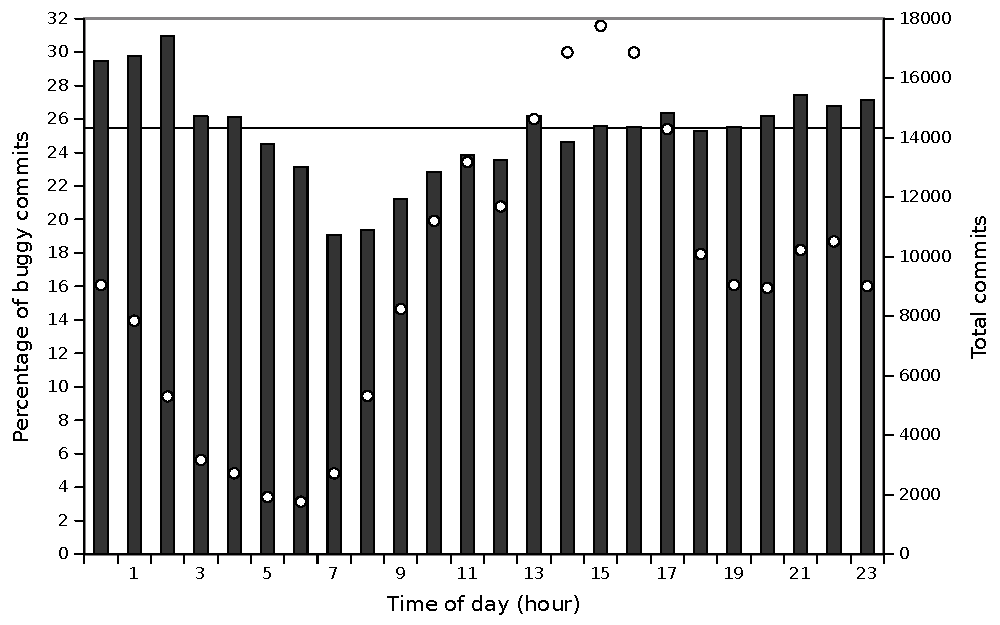
\includegraphics[width=\columnwidth]{linux-bugginess-hour.pdf}
}
\subfigure[PostgreSQL]{
 \label{fig-postgresql-bugginess-hour}
 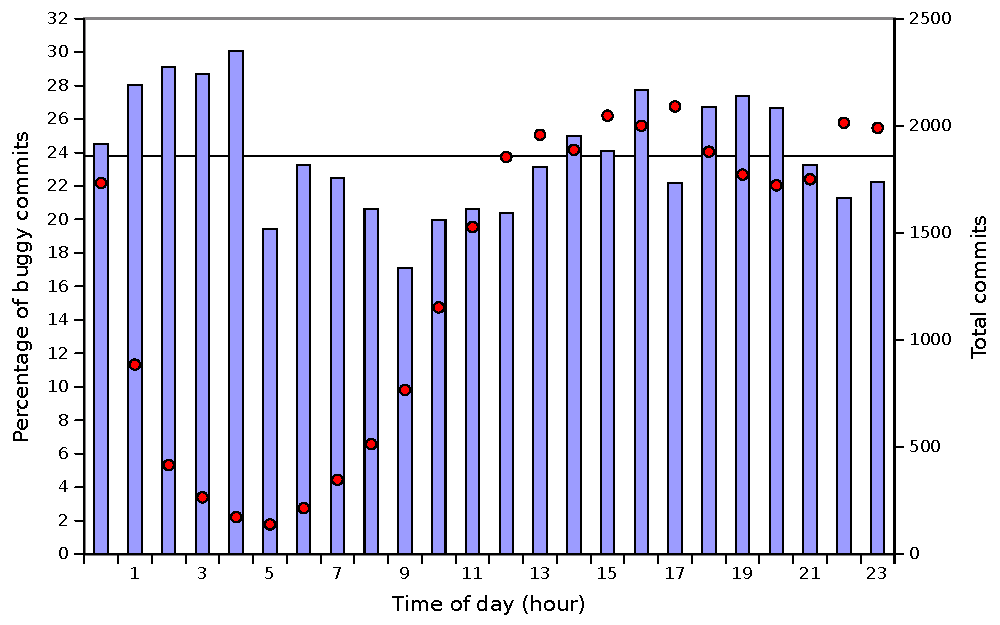
\includegraphics[width=\columnwidth]{postgresql-bugginess-hour.pdf}
}
\caption{\label{fig-bugginess-hour}Percentage of buggy commits (bars) and total number of commits (circles) versus time-of-day}
\end{figure*}

\begin{figure*}[tbh]
\centering
\subfigure[{Linux kernel}]{
 \label{fig-linux-introduction-hour}
 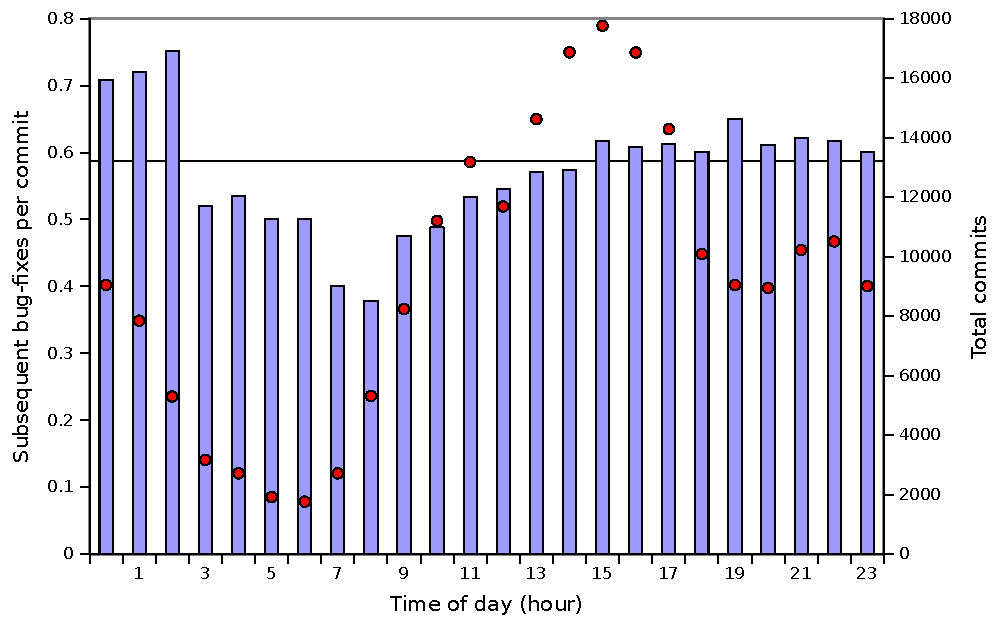
\includegraphics[width=\columnwidth]{linux-introductions-hour.pdf}
}
\subfigure[PostgreSQL]{
 \label{fig-postgresql-introduction-hour}
 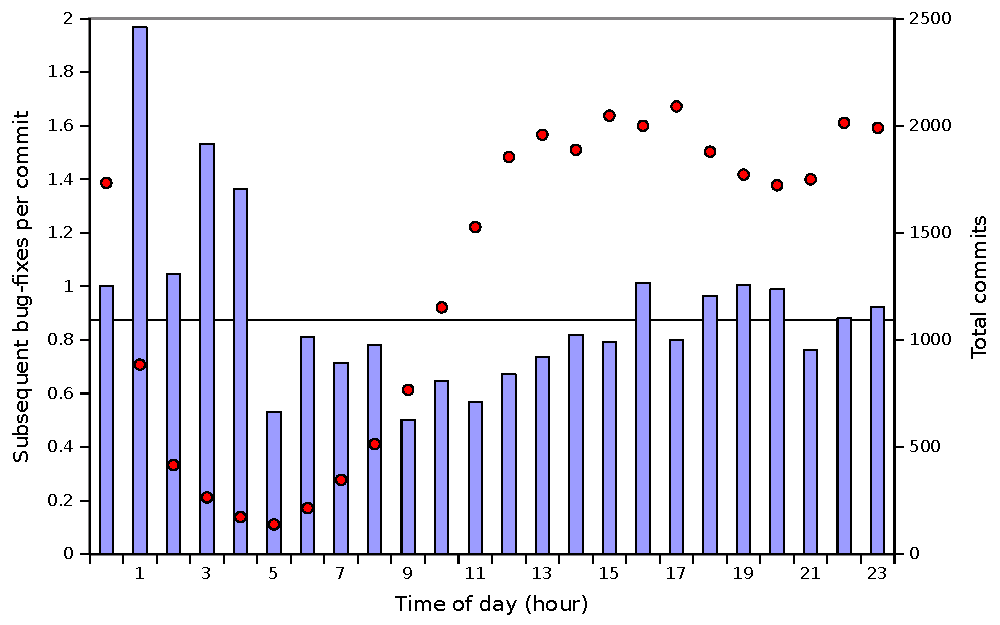
\includegraphics[width=\columnwidth]{postgresql-introductions-hour.pdf}
}
\caption{\label{fig-introduction-hour}Subsequent bug fixes per commit (bars) and
 total commits (circles) versus time-of-day}
\end{figure*}

%% \begin{figure*}[tbh]
%% \centering
%% \subfigure[{Linux kernel}]{
%% \label{fig-linux-severity-hour}
%% 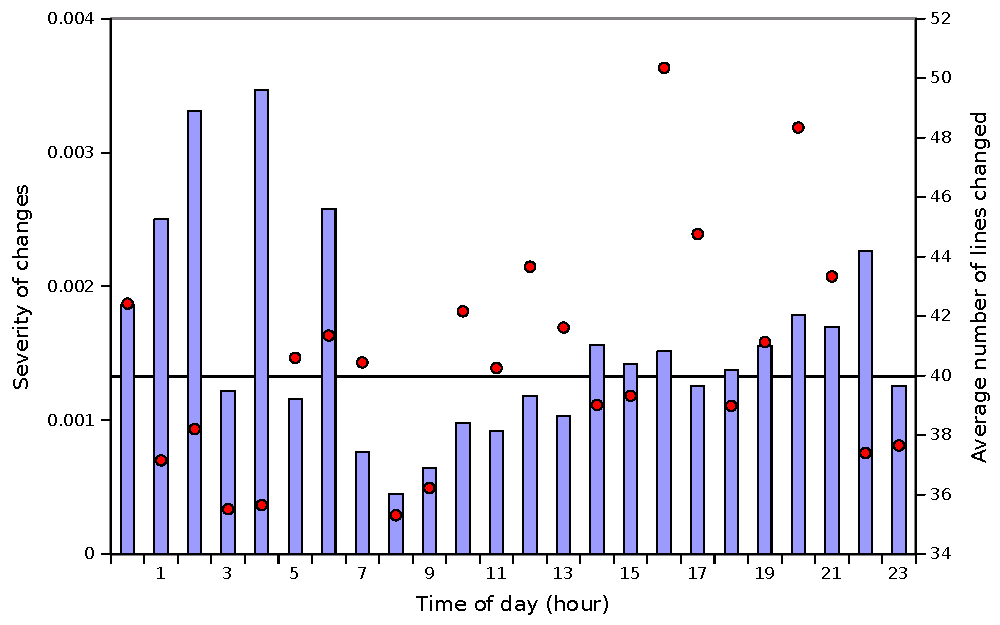
\includegraphics[width=\columnwidth]{linux-severity-hour.pdf}
%% }
%% \subfigure[PostgreSQL]{
%%  \label{fig-postgresql-severity-hour}
%%  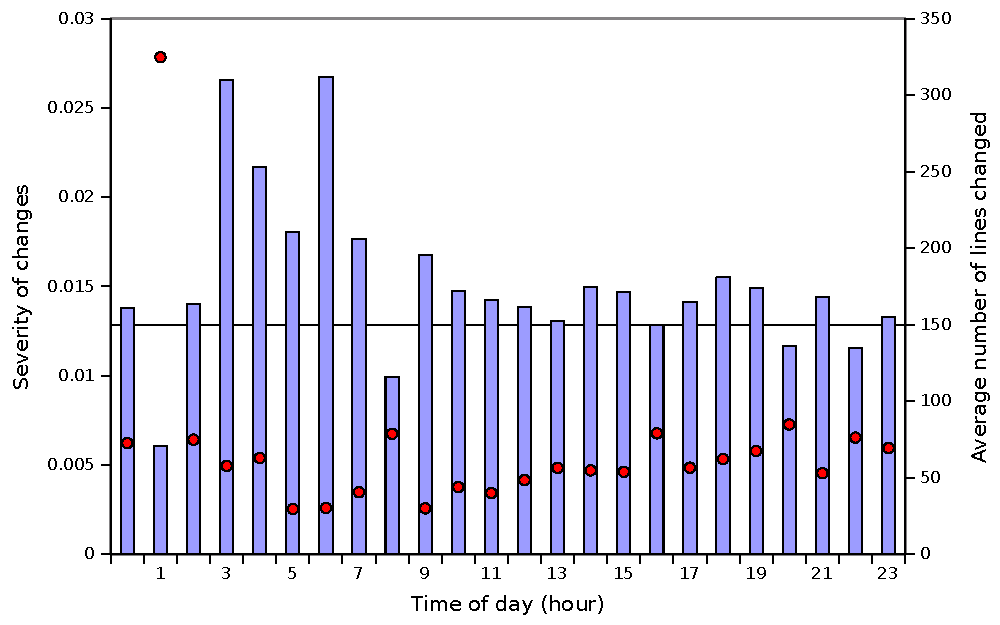
\includegraphics[width=\columnwidth]{postgresql-severity-hour.pdf}
%% }
%% \caption{\label{fig-severity-hour}Severity of changes (bars) and average number
%%  of lines per commit (circles) versus time-of-day}
%% \end{figure*}

\subsection{Time-of-day} 
\label{sec-time-of-day}

Figure~\ref{fig-bugginess-hour} presents our results correlating the time-of-day
of a commit with its bugginess. The graphs compare the time-of-day of each
commit, in the committer's local time on a 24-hour clock, to the percentage of
bug-introducing commits. The solid horizontal line
indicates the overall percentage of buggy commits in each project; bars
shorter than the line indicate that commits at that hour were less likely to be
buggy, while bars taller than the line indicate hours with more-buggy
commits. The graphs also contain the raw number of commits at each hour, 
indicated by circles.

%% While our principal metrics are the absolute count and percentage of
%% bug-introducing commits, we also present results of a third metric, \emph{bug
%% severity}. This metric attributes less weight to a large commit which
%% introduces a small number of bugs relative to its size, and more weight to small
%% commits which introduce relatively large numbers of bugs. We define bug severity
%% to be the number of bug introductions per changed non-comment lines of
%% code. Figure~\ref{fig-severity-hour} presents our data correlating severity of
%% changes, along with average commit size, with time-of-day.

Figure~\ref{fig-bugginess-hour}, which summarizes bugginess percentages, shows a
noticeable increase in the amount of commits which introduce a bug between 00:00
(midnight) and 04:00 (4 AM). After 04:00, commits tend to be less buggy than
average, gradually increasing until noon. In the Linux kernel, commits between
noon and midnight fluctuate around the average bugginess level, while the
PostgreSQL commits are generally above the average bugginess level between 16:00
(4 PM) and 20:00 (8 PM), and then below the average bugginess level between 20:00
(8 PM) and 00:00 (midnight). Figure~\ref{fig-introduction-hour}, which shows the
number of subsequent bug-fixing commits for each bug-introducing commit 
(indicating how difficult it was to correct a bug), follows the trends from
Figure~\ref{fig-bugginess-hour}. Note that even the smallest total number of
commits, for any hour, is 139 for PostgreSQL (and an order of magnitude higher
for the Linux kernel), so that all of the depicted bug introduction rates are
meaningful.

%% Figures~\ref{fig-linux-severity-hour} and~\ref{fig-postgresql-severity-hour}
%% show that the severity of late-night/early-morning changes (before 9 AM) is
%% surprisingly high, while there is no general trend in the average commit size.
%% The average size of Linux commits fluctuates quite a lot; the sizes of
%% PostgreSQL commits are more stable. For PostgreSQL, developers tend to commit
%% slightly smaller changes between 5 AM and noon, with a spike at 8 AM.

We also investigated correlations between the time-of-day and the number of
bug-fixing commits, rather than the bug-introducing commits that we showed
above. The proportion of total commits that are bug-fixing commits
stayed almost constant, independent of the hour; the graphs (not shown) have
exactly the same shape as that of the circles in
Figure~\ref{fig-bugginess-hour}. This suggests that the fact that a commit is
bug-fixing is independent of its other characteristics.

\begin{table}[tbh!]
\begin{center}
\small
\begin{tabular}{r|r|r}
\multicolumn{1}{c}{} & \multicolumn{2}{c}{{\bf P-value}} \\
\multicolumn{1}{c|}{{\bf Hour}} & \multicolumn{1}{c|}{{\bf Linux kernel}} &
\multicolumn{1}{c}{{\bf PostgreSQL}} \\
\hline
0  & 9.62E-18 & 0.245   \\
1  & 4.59E-18 & 0.00205 \\
2  & 1.62E-19 & 0.00748 \\
3  & 0.197    & 0.0382  \\
4  & 0.232    & 0.0348  \\
5  & 0.173    & 0.133   \\
6  & 0.0116   & 0.464   \\
7  & 1.56E-15 & 0.308   \\
8  & 2.62E-26 & 0.0494  \\
9  & 4.54E-20 & 3.80E-6 \\
10 & 3.25E-11 & 0.00108 \\
11 & 6.88E-6  & 0.00179 \\
12 & 6.13E-7  & 2.63E-4 \\
13 & 0.0255   & 0.258   \\
14 & 0.00447  & 0.114   \\
15 & 0.366    & 0.386   \\
16 & 0.436    & 2.40E-5 \\
17 & 0.00929  & 0.0456  \\
18 & 0.301    & 0.00176 \\
19 & 0.471    & 2.70E-4 \\
20 & 0.0695   & 0.00314 \\
21 & 4.91E-6  & 0.311   \\
22 & 0.00115  & 0.00433 \\
23 & 2.42E-4  & 0.0509  \\
\end{tabular}
\end{center}
\caption{\label{tbl-pvalues}Linux kernel and PostgreSQL bugginess p-values}
\end{table}

Table~\ref{tbl-pvalues} presents p-values evaluating the
statistical significance of the per-hour commit bugginess for
Linux and PostgreSQL.  The null hypothesis is that each
hour has the same probability as the overall bugginess for each
project.  Typically, a p-value less than 0.05 indicates that the null
hypothesis is rejected, and the corresponding result is considered to
be statistically significant.  Therefore, our p-value results show
that the differences in bugginess of different hours are statistically
significant. Concretely, the p-values allow us to conclude that
commits introduced between 00:00 (midnight) and 04:00 (4 AM) are
buggier than average with statistical significance.

%We only calculated p-values for bugginess since it is discrete, 
%an individual commit is either buggy or not.

\newpage
\paragraph{Discussion}

Code does not spontaneously improve if left to ``mature'' for 4 hours; 
our results do not indicate causation,
but instead demonstrate a correlation between code committed early in the 
morning and increased bugginess. We do not speculate about the cause
of this correlation; however, the results in Section~\ref{sec:toddev-exp}
imply that this correlation holds for both inexperienced and experienced
developers.
Our results do suggest that developers, being aware of such a 
correlation, may want to double-check code before performing
late-night commits (midnight--4:00 AM). It may also be
beneficial for version control systems or IDEs to warn developers about
the perils of late-night
commits. 
Our p-values indicate that our
observed bugginess differences between late-night/early-morning and all other commits are statistically significant.

Our results also suggest that tired developers (midnight--4 AM) are more likely to
miss corner cases in a pre-commit review (for PostgreSQL) or while finalizing
their patch (for the Linux kernel). Furthermore, we can observe that commits
before noon are least likely to be bug-introducing; perhaps committers are most
careful in those hours.

\begin{figure}[t!hb]
\begin{center}
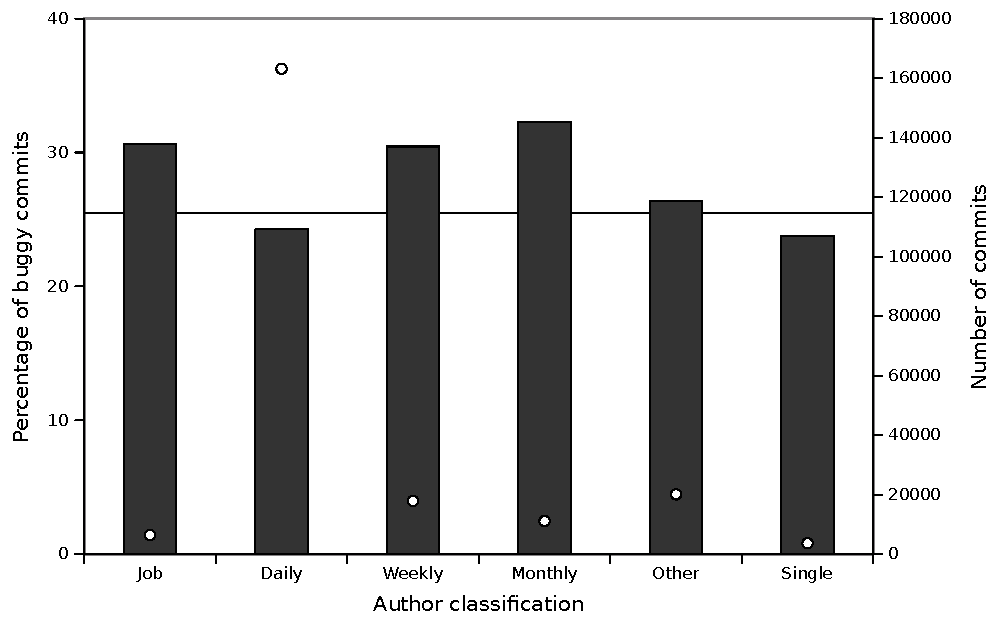
\includegraphics[width=\columnwidth]{linux-bugginess-author-class.pdf}
\end{center}
\caption{\label{fig-linux-bugginess-author-class}Linux percentage of buggy
 commits (bars) and number of commits (circles) versus author classification}
\end{figure}

\subsection{Developer Characteristics}
\label{sec-dev-char}

We next present our findings with respect to developers' commit frequency and
experience. Developers' commit frequency summarizes the frequency
of a developer's contributions to a project, while developer experience tracks
how long a developer has contributed to a particular project.

\subsubsection{Commit Frequency Classification} 

As we described in Section~\ref{sec:data}, one of the ways that we classify
developers is according to frequency, i.e. most-common interval between
consecutive commits---daily, weekly, monthly, other, or single. This
information is only interesting for the Linux kernel, as almost all (28/34) of
PostgreSQL's committers are daily. We computed the bugginess rates for each of
these classes of developers and plot author classification versus
bug-introduction percentage in
Figure~\ref{fig-linux-bugginess-author-class}. The graph also presents the
number of commits by each class. Note that the Linux kernel has 49 day job
authors, who provide quite a few of the total commits, 801 daily authors, who
account for the overwhelming majority of commits, 238 weekly, 288 monthly, 3562
other (less than 20 commits and more than 1 commit), and 3664 single-commit authors.

Our results show that the Linux kernel developers who commit changes daily, but
not as their day job, produce the largest number of commits and the smallest
number of bug-introducing commits, followed by the single-commit authors (whose
patches would presumably be simple or closely-reviewed). The day job, weekly,
and monthly committers all produce slightly more bug-introducing commits than
average.

\paragraph{Discussion}

A possible cause for the difference between day-job and daily committers is that
day-job developers might be required to make changes by their employers, while
the daily developers are motivated purely by interest, and unlikely to be
pressured to fix bugs on any particular schedule.

\begin{figure*}[tbh]
\centering
\subfigure[{Linux kernel}]{
 \label{fig-linux-bugginess-experience}
 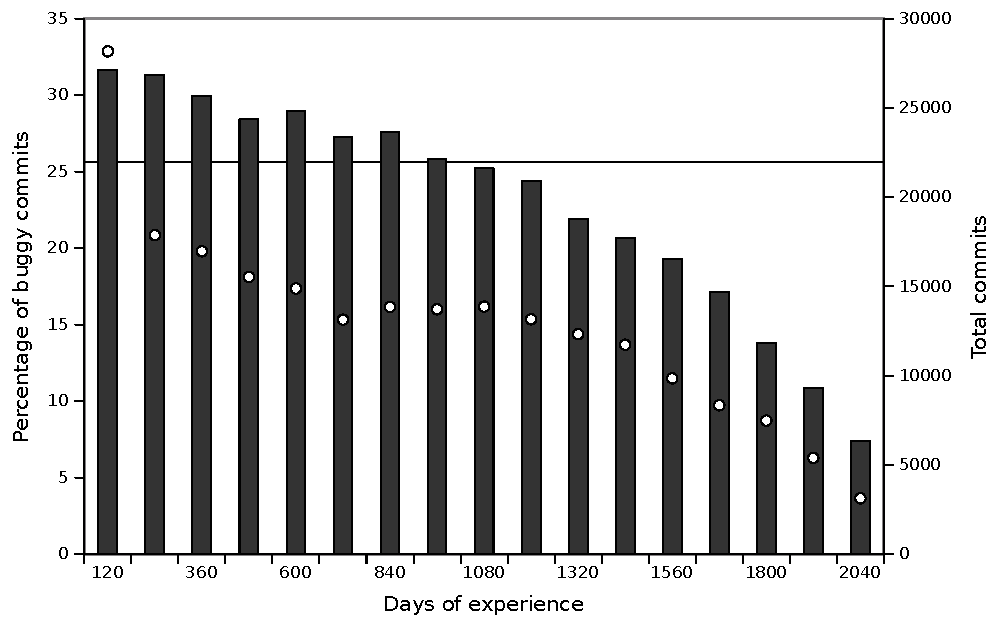
\includegraphics[width=\columnwidth]{linux-bugginess-experience.pdf}
}
\subfigure[PostgreSQL]{
 \label{fig-postgresql-bugginess-experience}
 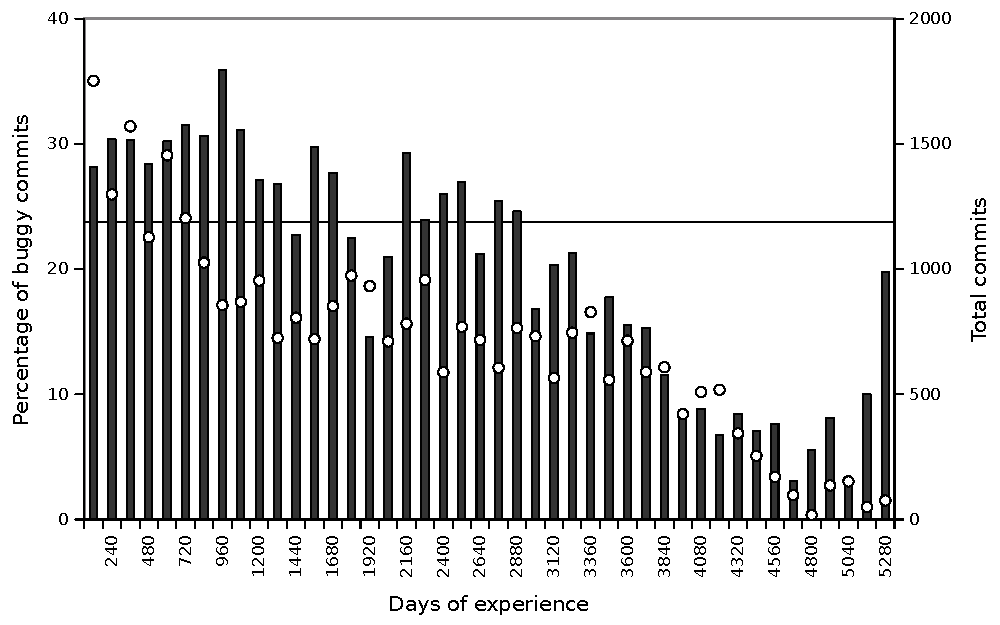
\includegraphics[width=\columnwidth]{postgresql-bugginess-experience.pdf}
}
\caption{\label{fig-bugginess-experience}Percentage of buggy commits (bars) and total number of commits (circles) versus author experience}
\end{figure*}

\subsubsection{Developer Experience}
\label{sec-dev-exp}

Figure~\ref{fig-bugginess-experience} compares author experience at time of
commit to the bugginess of the commit. It also presents the total number of
commits by author experience. Note that a plurality of Linux commits are by
authors with fewer than 120 days of experience. Both the Linux and PostgreSQL
data show that bugginess decreases with increased author experience. For Linux,
authors with at least 960 days of experience tend to produce commits that are
less buggy than average, while the similar point for PostgreSQL occurs at 3000
days. The PostgreSQL data also shows a spike at the right, which implies
surprisingly high bugginess in code recently committed by the original authors.

\paragraph{Discussion}

Our data shows that, in general, the more experienced the developers are, the
less likely that their commits are buggy. Without further data, this
correlation does not prove that the developer experience caused more experienced
programmers' commits to be less buggy. While we believe the above causation to
hold, other interpretations are possible; perhaps more experienced developers
wrote more complex code, whose bugs are harder to discover and less likely to be
reported. Nonetheless, our results show that, given the fact that a commit is
from a more experienced developer, one can be more confident about the
correctness of the commit. Such a correlation could be exploited to help predict
buggy code locations.

One can observe a decline in the total number of commits with experience.
We believe that this is due to our sliding scale for author experience.
Consider an author who has committed for 5 years. His or her commits do not
show up in a single circle at the 1800-day mark; instead, they are distributed
throughout the 5 years of the commits, so that a commit on the author's second
birthday gets reported as a commit at day 700. One would therefore expect
more commits from ``inexperienced'' developers, since all developers go through
an inexperienced phase, while only a small number of developers reach the
more experienced phase.

We do not understand the spike in percentage of buggy commits to the
right of the PostgreSQL graph. Possible reasons include the shift to
Git, which is a known historical event, or, more speculatively,
perhaps PostgreSQL recently undertook major ongoing architectural
revisions, carried out by the experienced developers.

\begin{figure*}[tbh]
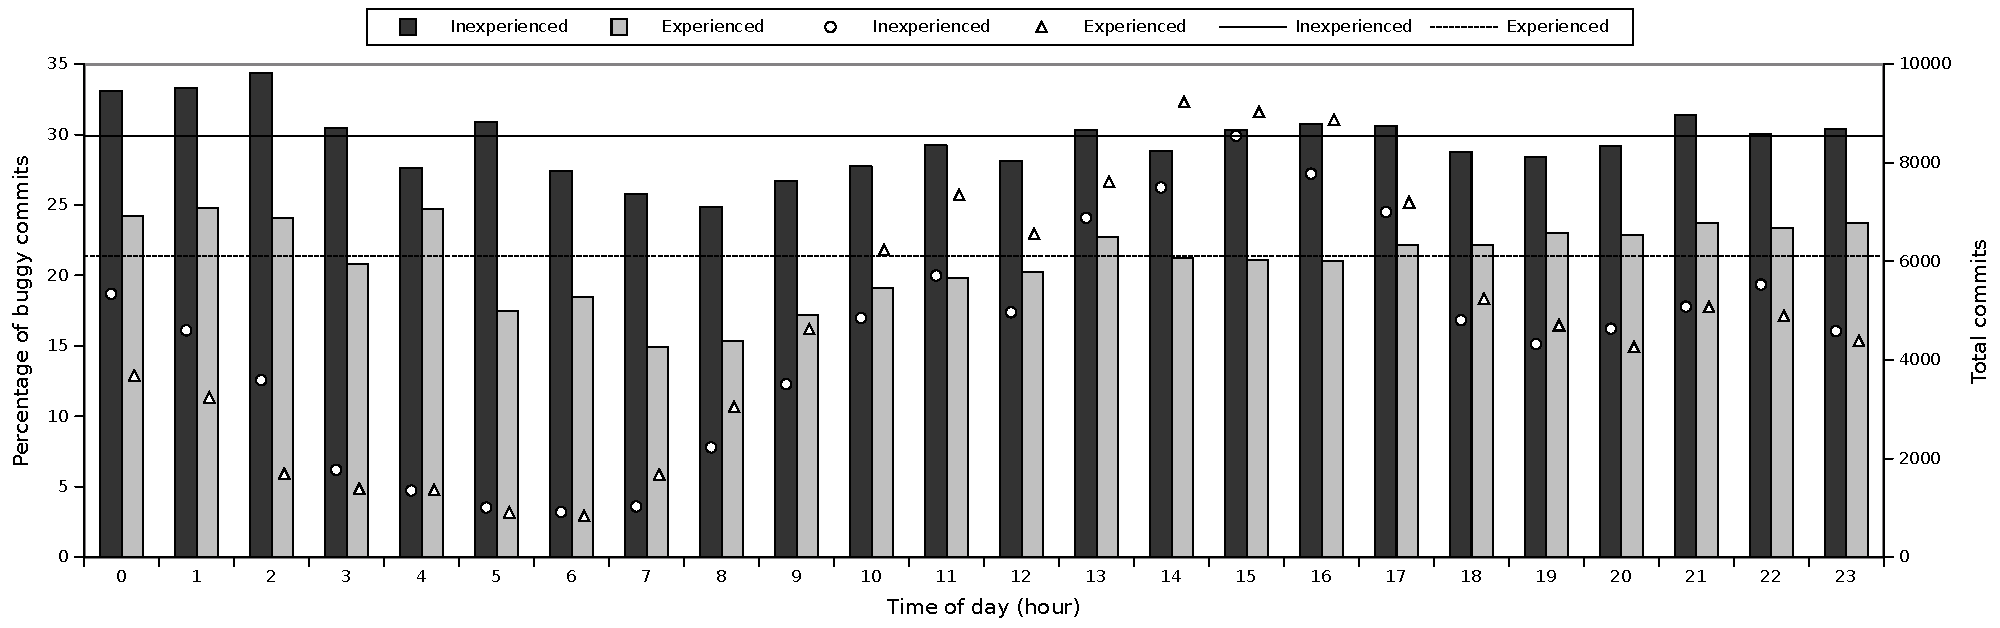
\includegraphics[width=\textwidth]{linux-bugginess-hour-experienced.pdf}
\caption{\label{fig-linux-bugginess-experienced}Percentage of buggy commits
 (bars) and total number of commits (circles/triangles) versus time-of-day for
 inexperienced and experienced Linux kernel developers}
\end{figure*}

\subsection{Combined Time-of-day and Experience}
\label{sec:toddev-exp}

Figure~\ref{fig-linux-bugginess-experienced} combines data from
Section~\ref{sec-time-of-day} and~\ref{sec-dev-exp} and correlates time-of-day
with commit bugginess for inexperienced and experienced developers,
plotted separately, for Linux. We used
a cutoff of 2 years to separate inexperienced and experienced developers; 
this cutoff divides the number of commits into two approximately-equal groups. 
Horizontal lines in the figure represent overall
bugginess. 

We can see that inexperienced developers tend to do more commits between
midnight and 2 AM than experienced developers, who do more commits between 8 AM
and 4 PM. However, there is a common trend for both; late night commits
(especially between midnight and 2 AM) are more buggy and early morning commits
(between 6 AM and noon) are less buggy.

\paragraph{Discussion}

This result suggests that the correlation between time-of-day versus
bugginess is independent of experience for Linux developers; it occurs
for both inexperienced and experienced developers. It also
shows that experienced developers are much less likely to commit a
bug; the average bugginess for experienced Linux developers is around
21\%, versus to 30\% for inexperienced developers. 

\begin{figure*}[tbh]
\centering
\subfigure[{Linux kernel}]{
 \label{fig-linux-bugginess-day}
 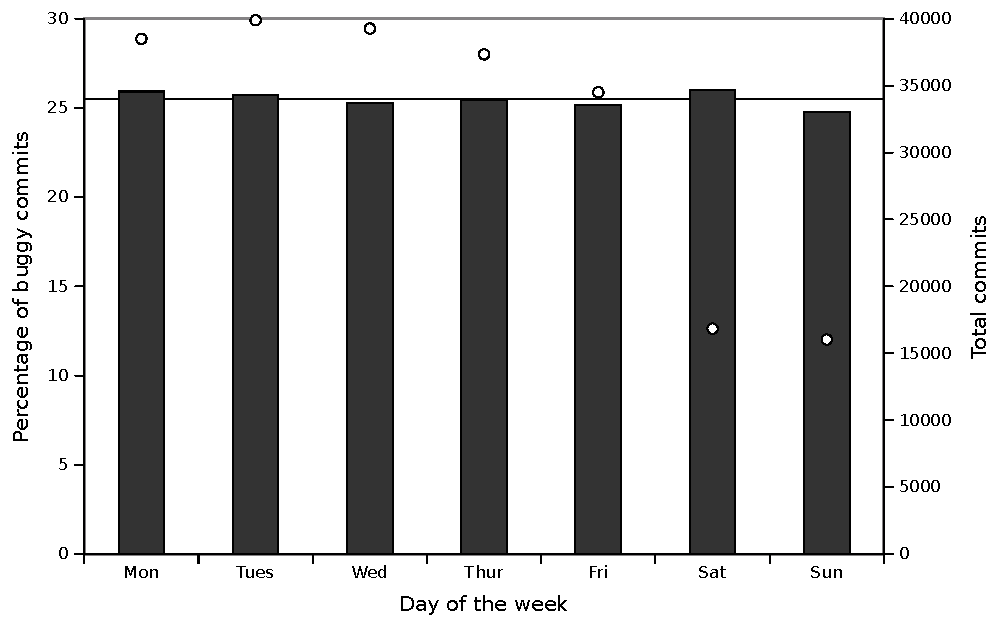
\includegraphics[width=\columnwidth]{linux-bugginess-day.pdf}
}
\subfigure[PostgreSQL]{
 \label{fig-postgresql-bugginess-day}
 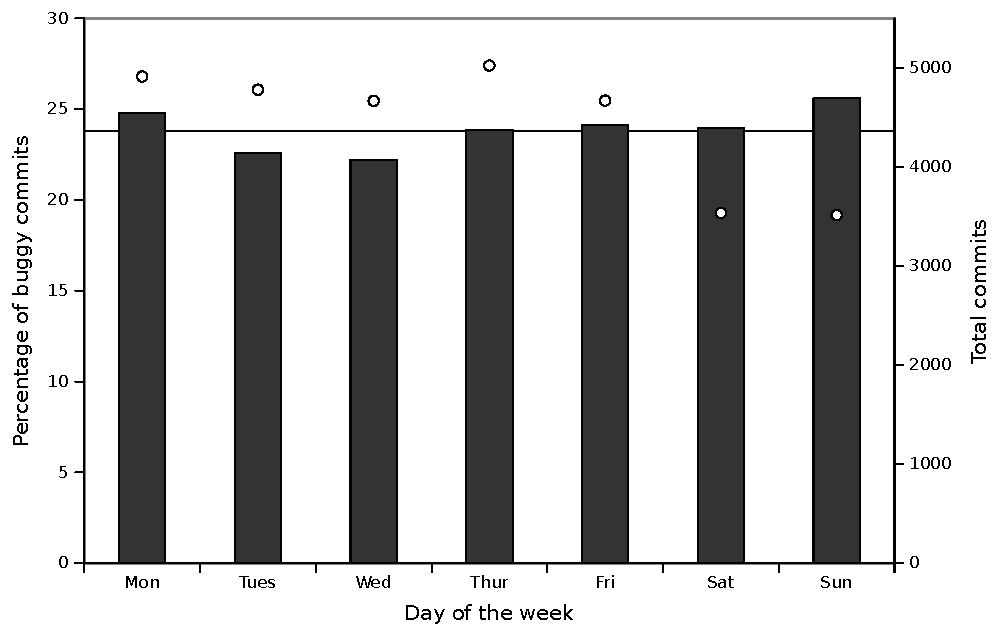
\includegraphics[width=\columnwidth]{postgresql-bugginess-day.pdf}
}
\caption{\label{fig-bugginess-day}Percentage of buggy commits (bars) and total
 commits (circles) versus day-of-week}
\end{figure*}

\begin{figure*}[tbh]
\centering
\subfigure[{Linux kernel}]{
 \label{fig-linux-introduction-day}
 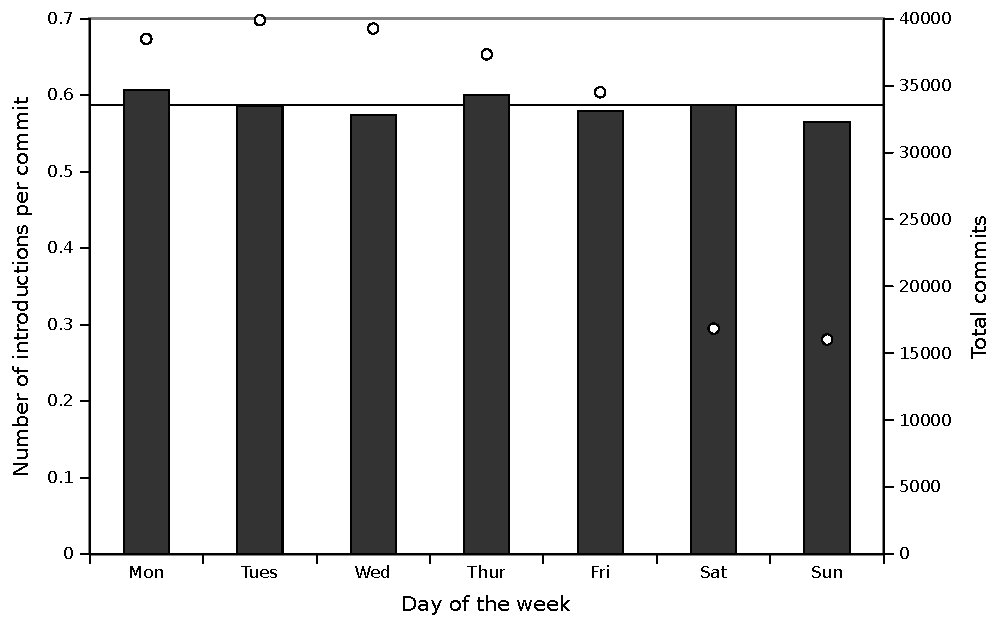
\includegraphics[width=\columnwidth]{linux-introductions-day.pdf}
}
\subfigure[PostgreSQL]{
 \label{fig-postgresql-introduction-day}
 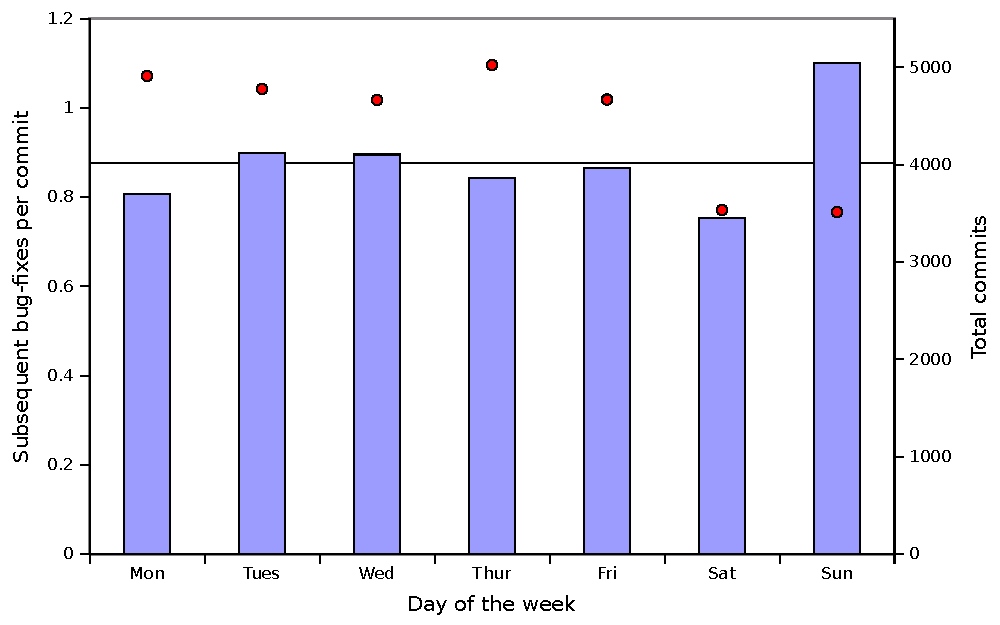
\includegraphics[width=\columnwidth]{postgresql-introductions-day.pdf}
}
\caption{\label{fig-introduction-day}Subsequent bug fixes per commit (bars) and total commits (circles) versus day-of-week}
\end{figure*}

%% \begin{figure*}[tbh]
%% \centering
%% \subfigure[{Linux kernel}]{
%%  \label{fig-linux-severity-day}
%%  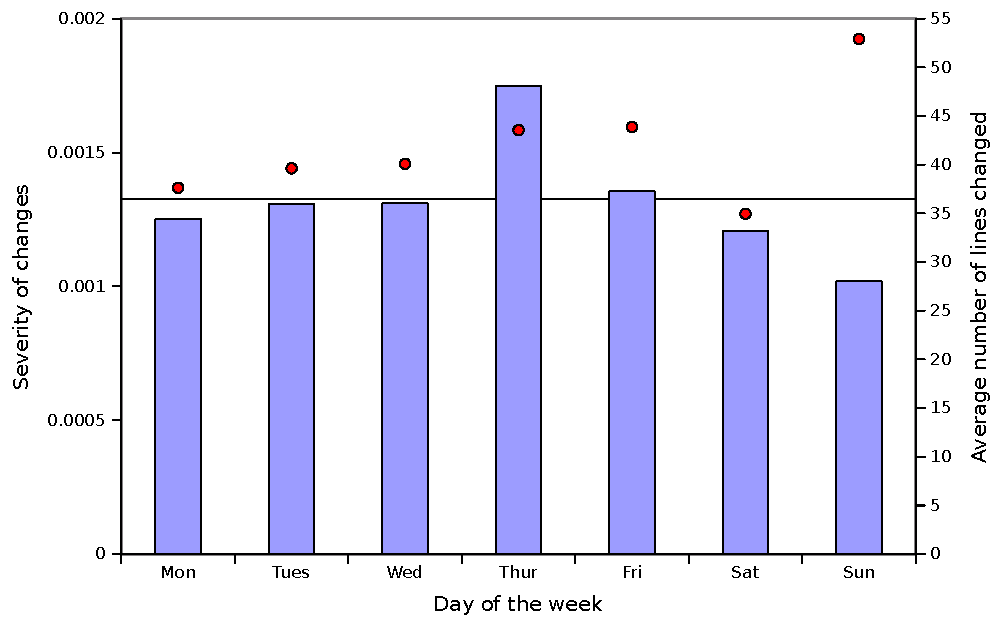
\includegraphics[width=\columnwidth]{linux-severity-day.pdf}
%% }
%% \subfigure[PostgreSQL]{
%%  \label{fig-postgresql-severity-day}
%%  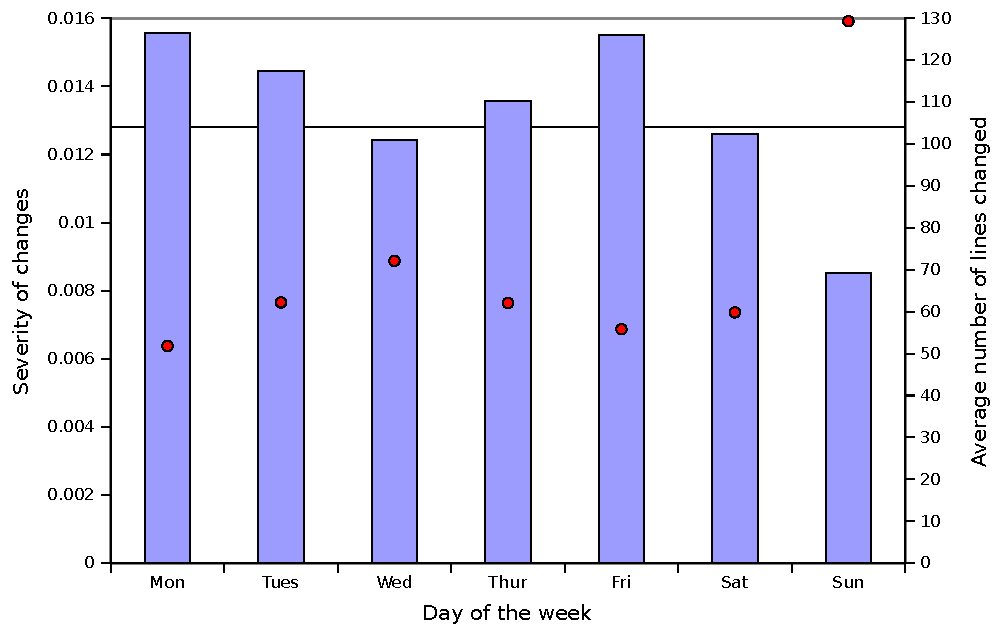
\includegraphics[width=\columnwidth]{postgresql-severity-day.pdf}
%% }
%% \caption{\label{fig-severity-day}Severity of changes (bars) and average number
%%  of lines per commit (circles) versus day-of-week}
%% \end{figure*}

\subsection{Day-of-week}
\label{sec-day-of-week}

Our next experiment attempted to replicate the results
in~\cite{sliwerski-msr-2005}, and correlates the day of the week of a commit with
its bugginess. Figure~\ref{fig-bugginess-day} compares the day of the week with
the bugginess of the commits on that day (bars), and also displays the total
number of commits per day (circles). Here, the solid horizontal line presents
the overall bugginess of all commits to each project.
Figure~\ref{fig-introduction-day} presents the number of subsequent bug-fixing
commits for each bug-introducing commit per day-of-week.%% , while
%% Figure~\ref{fig-severity-day} presents the severity of bugs per day-of-week, and
%% also presents the average sizes of commits.

Our results, which use a disjoint set of repositories from those
in~\cite{sliwerski-msr-2005}, found about the same bugginess and number of
introductions for each day in the Linux kernel repository, with the lowest
bugginess on Sunday and highest on Monday; for the PostgreSQL repository, we
observe a slight decrease in bugginess on Tuesday, and a noticeable increase on
Sunday. These results are statistically significant with a p-value less than
0.05. Note that, for Linux, Saturday and Sunday each have about half as many
commits as the other days of the week (commits peak on Tuesday and steadily
decrease through Friday). For PostgreSQL, commits fluctuate through the days of
the week and decrease to about 70\% of the weekday volume on the weekend. %% The
%% severity results do not show any particular trends, but we found that the
%% average number of lines per commit on Sunday was surprisingly large for both
%% Linux and PostgreSQL.

\paragraph{Discussion}

We found that commits on different days of week have about the same
bugginess, which does not agree with results from the prior study on two
different open source projects~\cite{sliwerski-msr-2005}. 
We also found that the bugginess per
day-of-week for commits varies for different software projects, implying that
bugginess prediction based on day-of-week may need to be calibrated on a 
per-project basis.

\subsection{Bug Lifetimes}
\label{sec-bug-lifetime}

Recall that the bug lifetime is the amount of time elapsed between the
bug-introducing commit and its bug-fixing commit. Figure~\ref{fig-bug-lifetime}
shows bug lifetimes for the Linux kernel and PostgreSQL, 
grouped in 120 day intervals. We found the average bug lifetime for the Linux
kernel is 1.38 years with a standard deviation of 1.35 years. The average bug
lifetime for PostgreSQL is 3.07 years with a standard deviation of 3.19
years. Note that the distribution of bug lifetimes is similar for both projects;
many bugs are fixed within a 120 day period and the overall lifetime appears to
decrease exponentially.

\paragraph{Discussion}

PostgreSQL may have a longer average bug lifetime due to being a smaller, less
complex project with a smaller user base. We found the sources of the long-time
bugs include race conditions, incorrect calculations and rare corner cases; such
cases are intuitively more likely to be found with a larger user base.

\begin{figure*}[tbh]
\centering
\subfigure[{Linux kernel}]{
 \label{fig-linux-bug-lifetime}
 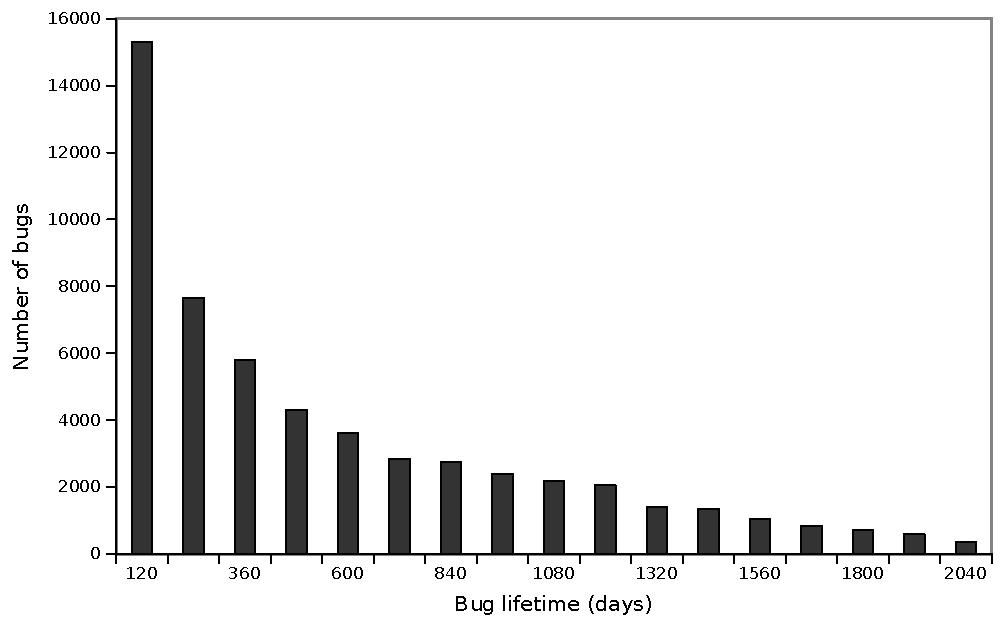
\includegraphics[width=\columnwidth]{linux-bug-lifetime.pdf}
}
\subfigure[PostgreSQL]{
 \label{fig-postgresql-bug-lifetime}
 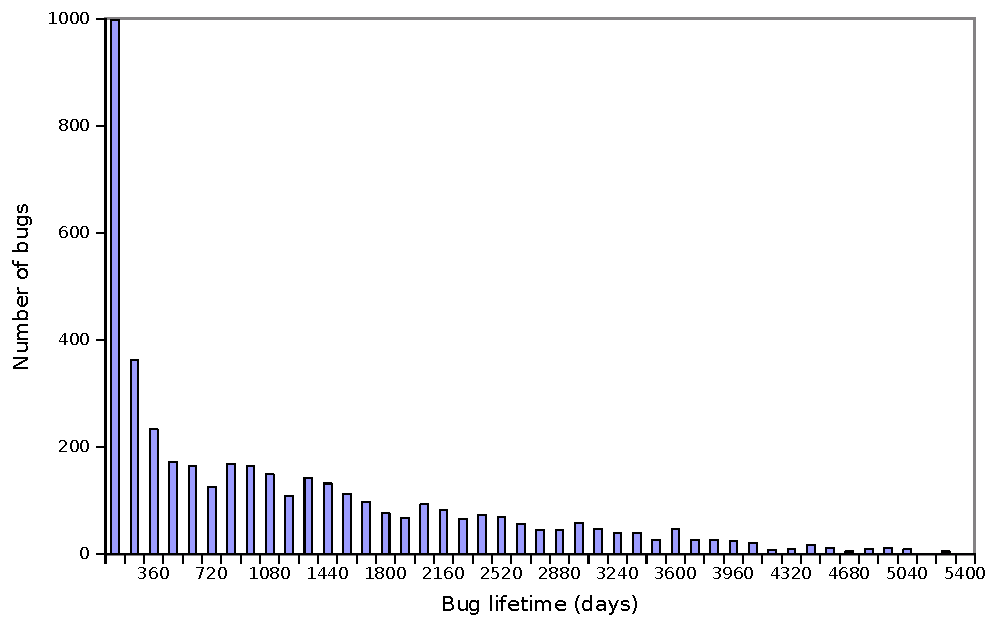
\includegraphics[width=\columnwidth]{postgresql-bug-lifetime.pdf}
}
\caption{\label{fig-bug-lifetime}Histogram of bug lifetime counts}
\end{figure*}

\subsection{Comment-only Commits}
\label{sec-comment-only}

A surprisingly large number of bug-fixing commits reported 0
changed lines of code. We performed a random sample on 50 of these commits for
each project and found that almost all of them only changed comments in the
source code, which we did not count as changed lines of code. For the Linux
kernel 2.15~$\pm$~0.10\%\footnote{We report the margin of error with 95\%
 confidence level.} of the bug-fixing commits (1,220
commits\footnote{Estimated based on the percentage of comment-only commits and
 the total number of commits.}) were on comments only. We followed the same
procedure for PostgreSQL and found 2.97~$\pm$~0.45\% (about 131 commits) of
bug-fixing commits were on comments only. These hundreds and thousands of
comment-only commits show that developers spend a nontrivial amount of time
purely maintaining the correctness of comments; these numbers don't even
consider the amount of time that developers incidentally update comments along
with the code.

%% We also noted that approximately 7.7\% of the bug fixes for Linux were purely
%% for comments, indicating that developers spend a non-trivial amount of time on
%% comments. For Linux, approximately 51\% of the changes do not include
%% additions. We therefore manually checked (a subsample of) the 49\% more
%% difficult cases to evaluate the effectiveness of our heuristic for additions.



\subsection{Validation} 
\label{sec-validation}

%% \begin{table}
%% \begin{center}
%% \begin{tabular}{rrrr}
%% & & \multicolumn{2}{c}{Predicted} \\
%% & & \multicolumn{1}{|c}{Fix} & \multicolumn{1}{c}{$\neg$Fix} \\ \cline{2-4}
%% \multirow{2}{*}{Actual} & \multicolumn{1}{c|}{Fix} & 48 & 18 \\
%%                         &  \multicolumn{1}{c|}{$\neg$Fix} & 7 & 127 \\
%% \end{tabular}
%% \end{center}
%% \caption{\label{tbl-linux-confusion}Linux kernel confusion matrix}
%% \end{table}

%% \begin{table}
%% \begin{center}
%% \begin{tabular}{rrrr}
%% & & \multicolumn{2}{c}{Predicted} \\
%% & & \multicolumn{1}{|c}{Fix} & \multicolumn{1}{c}{$\neg$Fix} \\ \cline{2-4}
%% \multirow{2}{*}{Actual} & \multicolumn{1}{c|}{Fix} &  30 & 12\\
%%                         &  \multicolumn{1}{c|}{$\neg$Fix} & 5 & 153 \\
%% \end{tabular}
%% \end{center}
%% \caption{\label{tbl-postgresql-confusion}PostgreSQL confusion matrix}
%% \end{table}





To validate our results, we estimated the precision and recall of our technique
for identifying bug-fixing commits on both projects. As our algorithm for
identifying the associated bug-introducing commits was a straightforward
application of git blame, we did not systematically verify its performance. (A
brief manual inspection of bug-introducing commits did not reveal any
anomalies.) For both projects, we randomly sampled 200 commits and manually
verified the results. Table~\ref{tbl-linux-confusion} and
\ref{tbl-postgresql-confusion} summarize our findings.

\begin{table}[tbh]
\centering
\small
\subfigure[{Linux kernel}]{
 \label{tbl-linux-confusion}
 \begin{tabular}{rrrr}
   & & \multicolumn{2}{c}{Predicted} \\
   & & \multicolumn{1}{|c}{Fix} & \multicolumn{1}{c}{$\neg$Fix} \\ \cline{2-4}
   \multirow{2}{*}{Actual} & \multicolumn{1}{c|}{Fix} & 48 & 18\\
                          &  \multicolumn{1}{c|}{$\neg$Fix} & 7 & 127 \\ \\
  \end{tabular}
}
\subfigure[PostgreSQL]{
  \label{tbl-postgresql-confusion}
  \begin{tabular}{rrrr}
    & & \multicolumn{2}{c}{Predicted} \\
    & & \multicolumn{1}{|c}{Fix} & \multicolumn{1}{c}{$\neg$Fix} \\ \cline{2-4}
    \multirow{2}{*}{Actual} & \multicolumn{1}{c|}{Fix} &  30 & 12\\
                            &  \multicolumn{1}{c|}{$\neg$Fix} & 5 & 153 \\ \\
  \end{tabular}
}
\caption{\label{tbl-confusion}Confusion matrices}
\end{table}


We evaluated the precision---that is, the proportion of identified bug-fixing
commits which do indeed fix bugs---and found that, for the Linux kernel, 48 of
the 55 bugs that we automatically identified as bug-fixing commits did indeed
fix bugs, while 7 did not; for PostgreSQL, 30 of 35 identified fixes were indeed
fixes. Some misclassifications included: 1) a commit message which fixed a merge
commit was classified as a fix; 2) apparently garbled commit messages which
included the keyword ``fix'' for no good reason; 3) changes which were reverted
(in the alleged ``fix'') but then re-added in a later version; 4) poor uses of
version control systems which included many different changes in a single
commit, including a fix as a small part of the commit; and 5) refactoring
changes, which moved or renamed functions; these could arguably be considered
to be fixes to a buggy initial design.

Our recall---the proportion of bug-fixing commits in the entire sample that our
technique identifies---is \linuxR for Linux and \postR for
PostgreSQL.
